\chapter{Microcontroller}
\label{ch:mcu}

To handle \gls{io} (not including output explained in Chapter \ref{chap:Output}), \vthreek is equipped with a \gls{mcu}.
This chapter will explain the reason for including this part, and its responsibilities.

\section{Silicon Labs EFM32 Giant Gecko}
A requirement for the assignment was to utilize a Silicon Labs EFM32 \gls{mcu} to act as an \gls{io} processor, listed in Table~\ref{tbl:non_func_req}.
The EFM is a \gls{soc}, and contains a 32-bit ARM Cortex-M3 processor, 1024kB flash memory and 128kB RAM \cite{efm32referencemanual}.

The Giant Gecko version was chosen for \vthreek.
The primary reason for choosing this variant of the EFM32 Gecko series, is that the EFM32GG DK3750 development kit was available for the team to test on from the beginning of the project.
It is the most powerful \gls{mcu} in the series, and thus provides the most possibilities \cite{efm32}.

\section{Responsibilities}
The \gls{mcu} does not have many responsibilities, and will in fact idle most of the time. The program flow is represented as a state diagram in Figure \ref{fig:mcu_state}.
Its primary tasks are:
\begin{itemize}
\item Load program instructions into \gls{sram}
\item Wait for button or joystick presses and react to these.
\item Controlling the status of the processor
\end{itemize}

\subsection{Loading program}
In order for the processor to do anything useful, a program is needed.
The program is contained within a header file in the \gls{mcu} flash.
After the MCU has booted and initialized the subsystems it utilizes, it will wait for a \texttt{Done} signal from the processor.
This signal tells the \gls{mcu} that the \gls{fpga} flash process has completed.
It is important to wait for this signal, because the state of any signal connected to the \gls{fpga} is undefined prior to flashing.
This could possibly interfere with the \gls{mcu} writing to \gls{sram}.

Once the \gls{fpga} is flashed and ready, the \gls{mcu} de-asserts the processor enable signal, to prevent it from start reading from \gls{sram} prematurely.
The \gls{mcu} then writes the program to \gls{sram}, starting at address \texttt{0x0000}, writing 16 bits at a time. The function responsible for this task is listed in \ref{fig:write_program}.
When complete, the processor enable signal is asserted, and the processor will begin fetching instructions.

\begin{figure}
	\centering
	\lstinputlisting[language=c, commentstyle=\color{blue}]{code/write_program.c}
	\label{fig:write_program}
	\caption{Function writing the program to SRAM.}
\end{figure}

\subsection{Buttons and joystick}
The board is equipped with two push buttons and a 5-way joystick, connected to the \gls{mcu}'s \gls{gpio} pins.
These inputs can be programmed to do anything, but was initially designed for controlling pan and zoom of the primitives.
A more useful functionality for one button was discovered to be soft resetting the processor.

When the processor is in normal operation, the \gls{mcu} does nothing, and enters Energy Mode 2, to save power.
When a button is pressed, an interrupt is generated, and the \gls{mcu} woken to handle the interrupt.

\begin{figure}[h!]
\centering 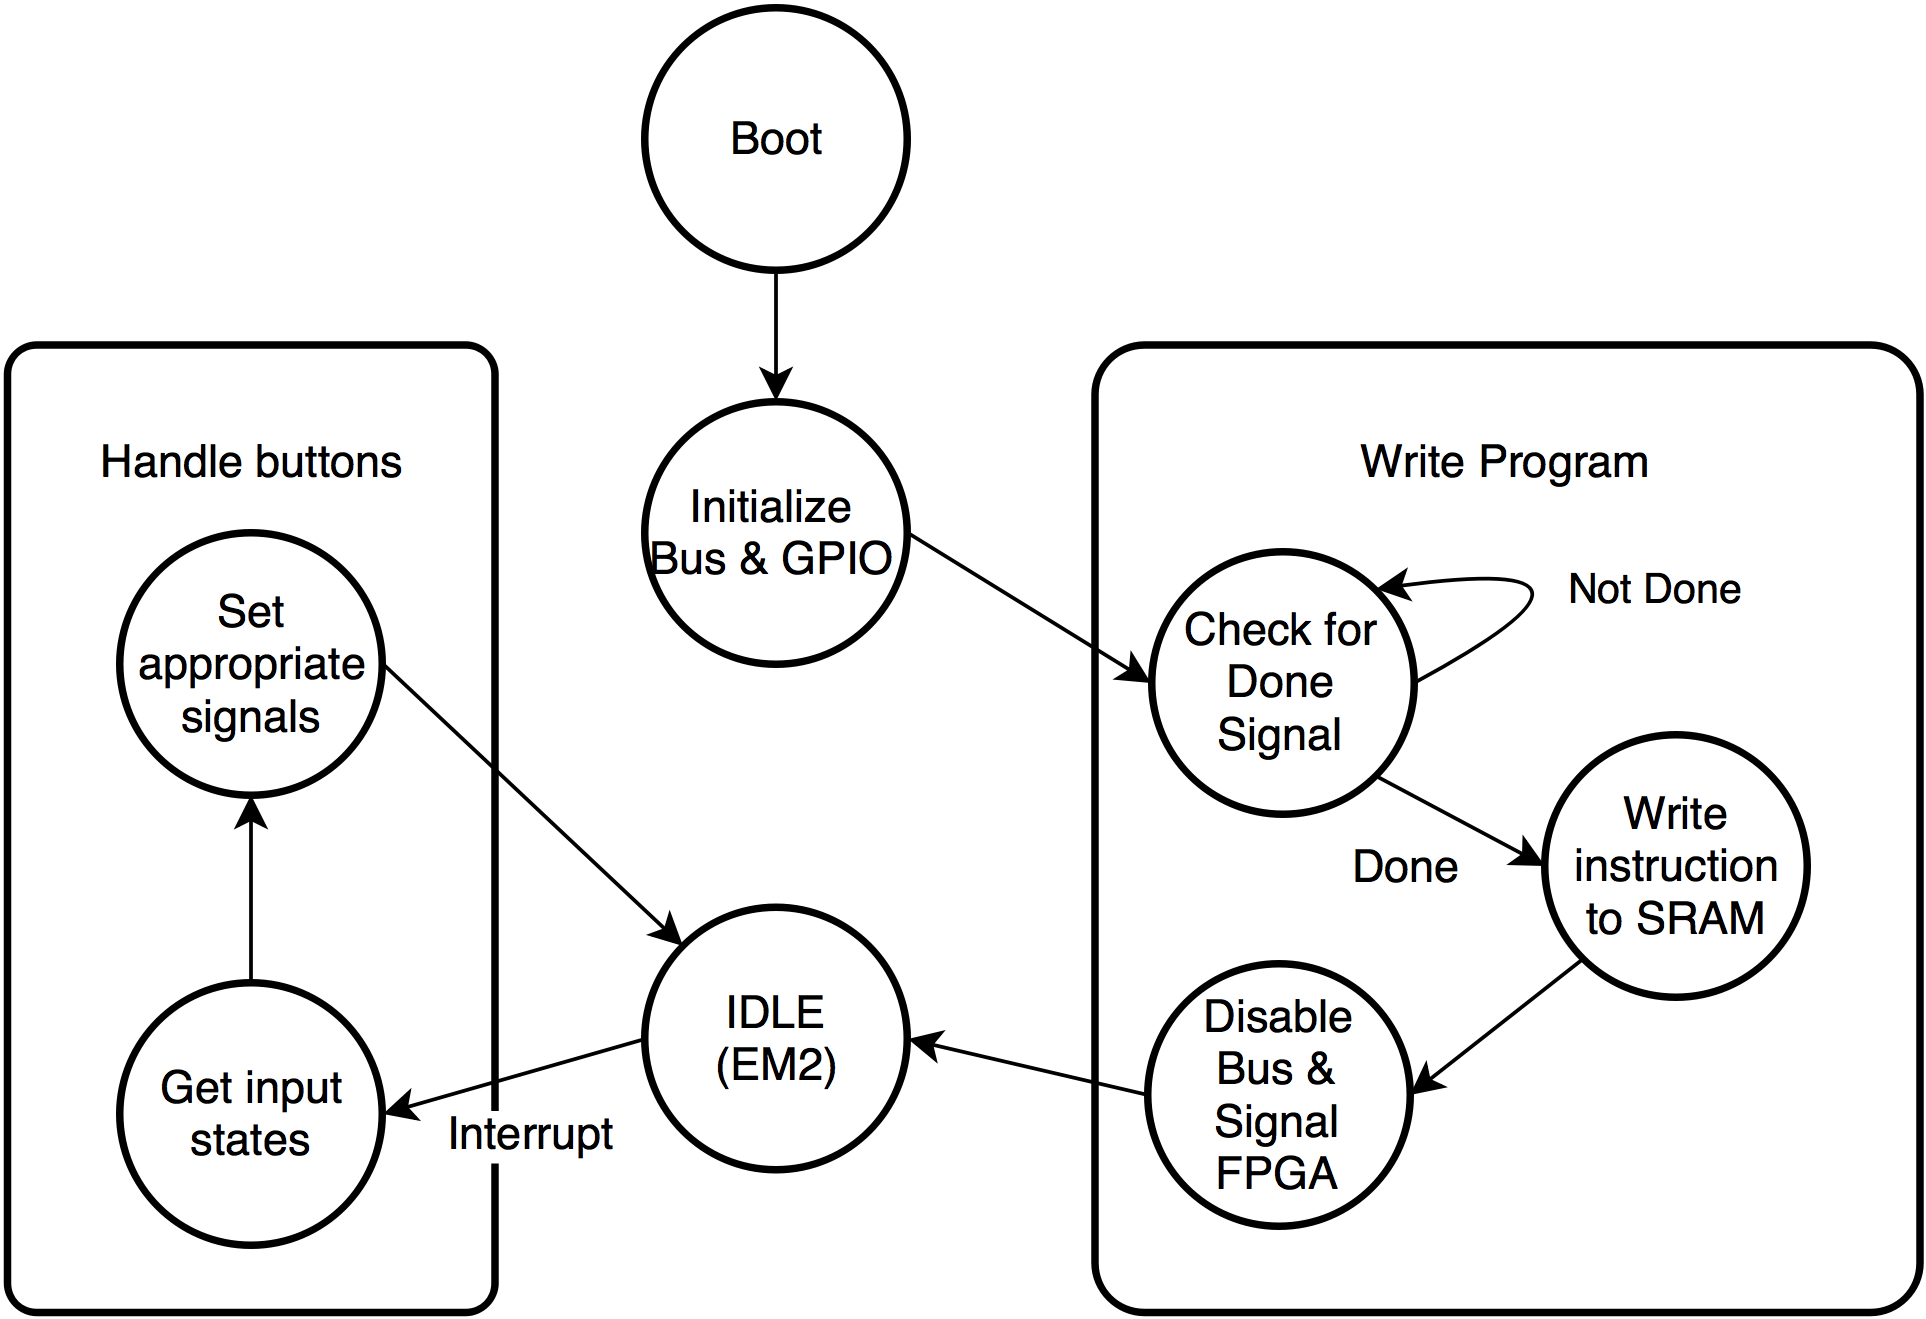
\includegraphics[width = 0.75\linewidth]{images/MCU_state.png}
\caption{The \gls{mcu} program represented as a state diagram}
\label{fig:mcu_state}
\end{figure}
